% TODO (template)
% - zrobić komendę \blocksection
% - opisać w komentarzach co robi który parametr
% - zrobić switch dla odstępu między kolumnami: proporcjonalny/absolutny
% - zmodyfikować "copyright" - będę jedynym autorem

%%%%%%%%%%%%%%%%%%%%%%%%%%%%%%%%%%%%%%
% LaTeX poster template
% Created by Nathaniel Johnston
% August 2009
% http://www.nathanieljohnston.com/2009/08/latex-poster-template/
%
% Modified by Paweł Kłeczek
% February 2017
%%%%%%%%%%%%%%%%%%%%%%%%%%%%%%%%%%%%%%

\documentclass[final,20pt]{beamer}
% 44 x 44 in
\usepackage[size=custom,width=111.76,height=111.76,scale=1,debug]{beamerposter}
% 40 x 44 in
%\usepackage[size=custom,width=101.6,height=111.76,scale=1,debug]{beamerposter}
\usepackage{graphicx}			% allows us to import images

%-----------------------------------------------------------
% Define the column width and poster size
%-----------------------------------------------------------

%\setlength{\paperwidth}{40in}
%\setlength{\paperheight}{44in}


\usepackage{calc}

\usepackage{siunitx}
\usepackage{paralist}
\usepackage{enumitem}
\usepackage{fp}
\usepackage{mathtools}
%\usepackage{amsfonts}
%\usepackage{amsmath}
\usepackage{caption}
%\usepackage[flushleft]{threeparttable}
%\usepackage{booktabs}
%\usepackage{makecell}
%\usepackage{footnote}
%\usepackage{array}
%\usepackage{tabularx}
\usepackage{subcaption}
%\usepackage{gensymb} % degree symbol

\usepackage{filecontents}

% Facilitate the conditional compilation
\usepackage{etoolbox}


\setbeamertemplate{caption}[numbered]

\captionsetup{subrefformat=parens}


\newlength{\sepwid}
\newlength{\onecolwid}
\newlength{\twocolwid}
\newlength{\threecolwid}

\newcommand{\interblockskip}{\vskip1.5ex}
\newcommand{\interlineskip}{\vskip0.8ex}

%\newlength{\twocolwidold}
%
\newcommand{\ncols}{3}

% 40 x 44 in
%\newcommand{\sepwidcoef}{0.03}

% 44 x 44 in
\newcommand{\sepwidcoef}{0.02}

%\newcommand{\sepwidcoef}{0.1}
\setlength{\sepwid}{\paperwidth*\real{\sepwidcoef}}
\FPeval{\onecolscale}{(1 - (\ncols + 1)*\sepwidcoef) / \ncols}
\setlength{\onecolwid}{\paperwidth*\real{\onecolscale}}
%
%\setlength{\twocolwidold}{0.464\paperwidth}
%\setlength{\threecolwid}{0.708\paperwidth}
\setlength{\twocolwid}{\onecolwid*\real{2}+\sepwid}
\setlength{\threecolwid}{\onecolwid*\real{3}+\sepwid*\real{2}}
%
\setlength{\topmargin}{-0.5in}
%
\usetheme{confposter}
\usepackage{exscale}

\newcommand{\blocksection}[1]{{\bfseries #1}}

\newlength{\groupwidth}
\newlength{\picwidth}
\newlength{\imgwidth}
\newlength{\imgheight}

% DEF : Math commands
\DeclarePairedDelimiter\abs{\lvert}{\rvert} % Requires `mathtools` package.
\newcommand{\argmin}{\operatornamewithlimits{arg \, min}}


%-----------------------------------------------------------
% Configure TikZ/PGFplots
%-----------------------------------------------------------

\usepackage{tikz}
\usepackage{pgfplots}
\usepackage{tikzscale}

\usetikzlibrary{calc,shapes,shadows,arrows,positioning,graphs}
\tikzset{>=latex}

\pgfplotsset{compat=1.8}
\pgfplotsset{minor grid style={dashed,black!15!white}}	
\pgfplotsset{major grid style={black!35!white}}	

\usepgfplotslibrary{groupplots}

\begin{filecontents}{resultplot.tikz}
\begin{tikzpicture}
%
%> Define X-axis labels
\newcommand{\AsenTick}{1}
\newcommand{\AspeTick}{2}
\newcommand{\ApreTick}{3}
\newcommand{\NfailedTick}{4}
%
%\newlength{\resultsplotwidth}
%\setlength{\resultsplotwidth}{.65\linewidth}
%
%\newlength{\resultsplotheight}
%\setlength{\resultsplotheight}{10cm}
%
%\newlength{\resultsplotwidth}
%\setlength{\resultsplotwidth}{.65\linewidth}
%
%\newlength{\resultsplotwidthbars}
\setlength{\resultsplotwidthbars}{0.65\linewidth}
%
%
\newcommand{\NfailedZero}{0.15}
%
\begin{groupplot}[
group style = {group size = 2 by 1, horizontal sep=0cm},
%
height = \imgheight,
%height = \imgheight,
%width = 1.3\resultsplotwidthbars,
%
major x tick style = transparent,
axis x line=bottom,
ymajorgrids = true,
yminorgrids = true,
%> Set spacing between bars within an individual (symbolic) coordinate.
ybar=0.2em,
ymin = 0,
scaled y ticks = false,
minor tick num=3,
axis line style={-},
xtick style={draw=none}, % Hide tick marks
]
%
%
\nextgroupplot[
width = .75\resultsplotwidthbars,
%width = .5\linewidth,
symbolic x coords={\AsenTick,\AspeTick,\ApreTick},
xticklabels={$\overline{\mathcal{A}_{\text{SEN}}}$, $\overline{\mathcal{A}_{\text{SPE}}}$,$\overline{\mathcal{A}_{\text{PRE}}}$},
xtick = data,
bar width=1em,
enlarge x limits=0.3,
%
axis y line*=left,
%
ylabel = {\%},
y label style={font=\bfseries},	
ymax=100,
%
legend to name=methods,
%		legend columns=1,
		legend cell align=left,
		legend style={
			at={(1.25,1)}, anchor=north east,
			column sep=1ex,
			inner sep=0.5em
		},
point meta=explicit symbolic
]
%
\addlegendimage{empty legend}
%
% FIXME: use values from stats_conf.tex!
% method: ABCD
\addplot[style={blue,fill=blue!50!white,mark=none}]
coordinates { (\AsenTick, 99) (\AspeTick, 71) (\ApreTick, 21) };
%	\node[above] at (axis cs:\NfailedTick,0) {0};
%
% method: XYZ
%\addlegendimage{empty legend}
\addplot[style={red,fill=red!50!white,mark=none}]
coordinates { (\AsenTick, 86) (\AspeTick, 90) (\ApreTick, 44) };

% method: proposed
\addplot[style={green!60!black, fill={rgb,5:green,2;black,1;white,2},mark=none}]
coordinates { (\AsenTick, 140) (\AspeTick, 120) (\ApreTick, 101) };
%

\coordinate (top) at (rel axis cs:1.5,0.5);% coordinate at top of the first plot


\addlegendentry{\hspace{-.6cm}\textbf{Method}}
\addlegendentry{ABCD~\cite{ABCD}}
\addlegendentry{XYZ~\cite{XYZ}}
\addlegendentry{proposed}	
%
%
\nextgroupplot[
%width = .25\resultsplotwidthbars,
width = .25\resultsplotwidthbars,
symbolic x coords={\NfailedTick},
xticklabels={{\# failed}},
xticklabel style = {font=\bfseries},
xtick = data,
bar width=1em,
enlarge x limits=0.3,
%
axis y line*=right,
%
ylabel = {Count},
y label style={font=\bfseries},	
ymax=50,
point meta=explicit symbolic	
]
%
%\addlegendimage{empty legend}
%
% method: ABCD
\addplot[style={blue,fill=blue!50!white,mark=none}]
coordinates { (\NfailedTick, \NfailedZero) };
%	\node[above] at (axis cs:\NfailedTick,0) {0};

% method: XYZ
%\addlegendimage{empty legend}
\addplot[style={red,fill=red!50!white,mark=none}]
coordinates { (\NfailedTick, 12) };

% method: proposed
\addplot[style={green!60!black, fill={rgb,5:green,2;black,1;white,2},mark=none}]
coordinates { (\NfailedTick, \NfailedZero) };
%
%
%
\end{groupplot}
%	
%	\path (top)--(bot) coordinate[midway] (group center);
%	\node[above,rotate=90] at (group center -| current bounding box.west) {throughput};
%	\node[right=1em,inner sep=0pt] at(group center -| current bounding box.east) {\pgfplotslegendfromname{methods}};
\node[anchor = east, right=1em, inner sep=0pt] at(top) {\pgfplotslegendfromname{methods}};

\end{tikzpicture}
\end{filecontents}

%-----------------------------------------------------------
% Define colours (see beamerthemeconfposter.sty to change these colour definitions)
%-----------------------------------------------------------

\setbeamercolor{block title}{fg=ngreen,bg=white}
\setbeamercolor{block body}{fg=black,bg=white}
\setbeamercolor{block alerted title}{fg=white,bg=dblue!70}
\setbeamercolor{block alerted body}{fg=black,bg=dblue!10}

% -- Use a solid line as the separator between block title and block body.

%\colorlet{separation rule}{structure!40}

%\setbeamertemplate{blocks}[rectangles][shadow=true]
%\makeatletter
%\pgfdeclareverticalshading[lower.bg,upper.bg]{bmb@transition}{200cm}{%
%	color(0pt)=(separation rule); color(2pt)=(separation rule); color(4pt)=(separation rule)}
%\makeatother

%-----------------------------------------------------------
% Results
%-----------------------------------------------------------

\newcommand{\numel}[1]{{\mid#1\mid}}

\FPeval{\nwsisubc}{62}
\FPeval{\nwsiscmuj}{16}
\FPeval{\nwsisumch}{10}
\FPeval{\nwsis}{clip(\nwsisubc + \nwsiscmuj + \nwsisumch)}

\FPeval{\setallpropnFailed}{0}
\FPeval{\setallpropAsenmean}{0.8737}
\FPeval{\setallpropAspemean}{0.9471}
\FPeval{\setallpropApremean}{0.5651}
\FPeval{\setallpropAsenmed}{0.9672}
\FPeval{\setallpropAspemed}{0.9797}
\FPeval{\setallpropApremed}{0.6539}
\FPeval{\setallpropAseniqr}{0.0939}
\FPeval{\setallpropAspeiqr}{0.0554}
\FPeval{\setallpropApreiqr}{0.4269}


\FPeval{\asenpropperc}{\setallpropAsenmean * 100}
\FPeval{\aspepropperc}{\setallpropAspemean * 100}
\FPeval{\aprepropperc}{\setallpropApremean * 100}

\newcommand{\dispstat}[1]{\num[round-mode=places,round-precision=2]{#1}}
\newcommand{\dispperc}[1]{\SI[round-mode=places,round-precision=0]{#1}{\percent}}

%-----------------------------------------------------------
% Name and authors of poster/paper/research
%-----------------------------------------------------------

\title{Automated epidermis segmentation in histopathological images\linebreak of human skin stained with hematoxylin and eosin}

\author[shortname]{Pawe\l{} K\l{}eczek \inst{1} \and Grzegorz Dyduch \inst{2} \and Joanna Jaworek-Korjakowska \inst{1} \and Ryszard Tadeusiewicz \inst{1}}

\institute[shortinst]{%
\inst{1} AGH University of Science and Technology, Department of Automatics and Biomedical Engineering, Krakow, Poland %
\and %
\inst{2} Jagiellonian University Medical College, Department of Pathomorphology, Krakow, Poland%
}

%-----------------------------------------------------------
% Start the poster itself
%-----------------------------------------------------------

\titlegraphic{\vspace{8cm}}% to push the other text to the top

\newtoggle{GFXDEBUG}
\togglefalse{GFXDEBUG}
%\toggletrue{GFXDEBUG}

\newtoggle{DETAILEDPLOT}
\toggletrue{DETAILEDPLOT}
%\togglefalse{DETAILEDPLOT}

% \draftgraphics - a switch do disable/enable draft frames instead of the actual graphics (to speed-up the rendering process)
\iftoggle{GFXDEBUG}{
	% Debug ON
	\newcommand{\draftgraphics}{draft}
}{
	% Debug OFF
	\newcommand{\draftgraphics}{}
}

% START

\begin{document}
\begin{frame}[t]
	\newlength{\logosvoffset}
	\setlength{\logosvoffset}{-9.5cm}
	%	
	\newlength{\logoshoffset}
	\setlength{\logoshoffset}{9cm}
	
	\tikz [remember picture,overlay]
	\node at
	([xshift=\logoshoffset, yshift=\logosvoffset]current page.north west) 
	%	([xshift=7cm, yshift=-9cm]current page.north west) 
	{
\includegraphics[width=8cm]{images/logos/spie_logo.png}};
	
	\tikz [remember picture,overlay]
	\node at
	([xshift=-\logoshoffset, yshift=\logosvoffset]current page.north east) 
	%	([xshift=-7cm, yshift=-9cm]current page.north east) 
	{
\includegraphics[width=8cm]{images/logos/agh_logo.jpg}};
	
	\vspace*{-3cm}
	
	\begin{columns}[t]
	\begin{column}{\sepwid}\end{column}
	%
	\begin{column}{\onecolwid}
		\begin{alertblock}{Objectives}
		\textbf{The aim if our project was to provide students and employees of AGH-UST with a nice-looking conference poster template.}
		\end{alertblock}  
		%  	
		\interblockskip
		%
		\begin{block}{Introduction}
		 	Just a few words of introduction. Not too many, 'cause TLDR...
		%
		\vspace*{-0.4cm}
		\begin{columns}
			\setlength{\imgheight}{10cm}
			
			\begin{column}[T]{.45\textwidth}
				\centering
				\begin{figure}[h]
					\centering
					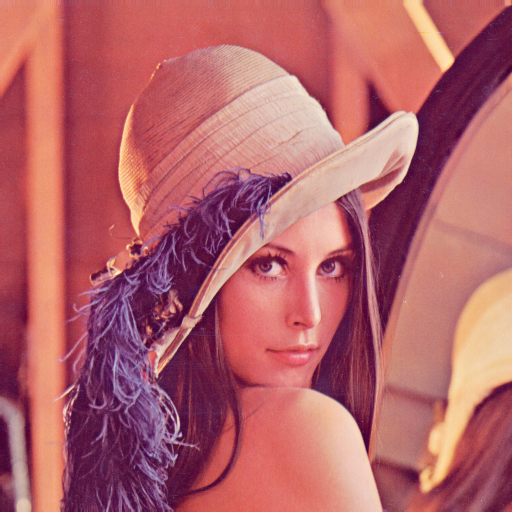
\includegraphics[\draftgraphics,height=\imgheight]{images/lenna.png}
					%
					\caption{\label{fig:skin_slide} Lena S\"oderberg~\cite{Lenna}.}
				\end{figure}
			\end{column}
			\begin{column}[T]{.45\textwidth}
				\centering
				\begin{figure}[h]
					\centering
					
\includegraphics[\draftgraphics,height=\imgheight]{images/dummy.png}
					%
					\caption{\label{fig:pipeline_whole} The proposed epidermis segmentation pipeline.}
				\end{figure}			
			\end{column}
		\end{columns}
			\end{block}
		%
		\interblockskip
		%
		\begin{block}{Method}

			Yet another block, but this time it's often desirable to split it into smaller subsections...
			
			\interlineskip
			
			% Add a label for easier navigation.
			% SEC : Section #1
			\blocksection{Section One}
			
			And here is an equation:
			\begin{equation}
				\label{eq:luma}
				\mathrm{Y} = 0.299 \, I_\mathrm{R} + 0.587 \, I_\mathrm{G} + 0.114 \, I_\mathrm{B}
				,
			\end{equation}
			but I have no idea if it makes sense to anyone.
			
			\interlineskip
			
			% SEC : Section #1
			\blocksection{Section Two}
			
			Just some more text... but wait! There is also a nice figure with subfigures~(Fig.~\ref{fig:subfigures}).

			\interlineskip

			\begin{figure}[h]
				\centering	
				\setlength{\imgheight}{8cm}
				
				\setlength{\fboxsep}{0pt}%
				\setlength{\fboxrule}{1pt}%	
				
				\begin{subfigure}[c]{0.45\textwidth}
					\centering
					\fbox{
\includegraphics[\draftgraphics,width=\linewidth]{images/dummy.png}}
					\caption*{\label{fig:subfig_x} X}
				\end{subfigure}
				\begin{subfigure}[c]{0.45\textwidth}
					\centering
					\fbox{
\includegraphics[\draftgraphics,width=\linewidth]{images/dummy.png}}
					\caption*{\label{fig:subfig_y} Y}
				\end{subfigure}
				
				% TODO: add subrefs
				\caption{\label{fig:subfigures} Subfigures.}
			\end{figure}	
		
			The Figure~\ref{fig:subfig_x} is IMHO the best one.
			
			\begin{figure}[h]
				\centering	
				\setlength{\imgheight}{5cm}
				\setlength{\groupwidth}{.225\linewidth}
				
				\setlength{\fboxsep}{0pt}%
				\setlength{\fboxrule}{1pt}%	
				
				\begin{subfigure}[c]{\groupwidth}
					\centering
					\fbox{
\includegraphics[\draftgraphics,width=\linewidth]{images/dummy.png}}
					\caption*{\label{fig:groupwidth_1} $A_1$}
				\end{subfigure}
				\begin{subfigure}[c]{\groupwidth}
					\centering
					\fbox{
\includegraphics[\draftgraphics,width=\linewidth]{images/dummy.png}}
					\caption*{\label{fig:groupwidth_2} $A_2$}
				\end{subfigure}
				\begin{subfigure}[c]{\groupwidth}
					\centering
					\fbox{
\includegraphics[\draftgraphics,width=\linewidth]{images/dummy.png}}
					\caption*{\label{fig:groupwidth_3} $A_3$}
				\end{subfigure}
				
				\caption{\label{fig:groupwidth} Groupwidth property.}
			\end{figure}				
									
		\end{block}		
	\end{column}
	%
	%
	\begin{column}{\sepwid}\end{column}
	%
	%
	\begin{column}{\twocolwid}
		\begin{columns}[t,totalwidth=\twocolwid]
			\begin{column}{\onecolwid}
				\begin{exampleblock}{}
					% SEC : Stain concentrations analysis
					\blocksection{Section Three}
					
					See? I don't need this fancy headers on top on each block. I can use an \textit{Example block} and yes -- just continue the previous block! Oh... and take a look on Figure~\ref{fig:plots} where you have examples of good-looking plots.
					
					\interlineskip

					\begin{figure}[h]
						\centering	
						\setlength{\imgheight}{7cm}
						\setlength{\groupwidth}{.45\linewidth}
						
						%> Configure collagen peak
\pgfmathsetmacro{\xoA}{0.3}
\pgfmathsetmacro{\yoA}{0.5}
%
\pgfmathsetmacro{\sigmaXA}{0.05}
\pgfmathsetmacro{\sigmaYA}{0.15}
\pgfmathsetmacro{\thetaA}{10}
%
\pgfmathsetmacro{\aA}{cos(\thetaA)^2/(2*\sigmaXA^2) + sin(\thetaA)^2/(2*\sigmaYA^2)}
\pgfmathsetmacro{\bA}{-sin(2*\thetaA)/(4*\sigmaXA^2) + sin(2*\thetaA)/(4*\sigmaYA^2)}
\pgfmathsetmacro{\cA}{sin(\thetaA)^2/(2*\sigmaXA^2) + cos(\thetaA)^2/(2*\sigmaYA^2)}
%
\pgfmathsetmacro{\fcA}{1.0}

%> Configure epidermis peak
\pgfmathsetmacro{\xoE}{0.6}
\pgfmathsetmacro{\yoE}{0.4}
%
\pgfmathsetmacro{\sigmaXE}{0.3}
\pgfmathsetmacro{\sigmaYE}{0.2}
\pgfmathsetmacro{\thetaE}{20}
%
\pgfmathsetmacro{\aE}{cos(\thetaE)^2/(2*\sigmaXE^2) + sin(\thetaE)^2/(2*\sigmaYE^2)}
\pgfmathsetmacro{\bE}{-sin(2*\thetaE)/(4*\sigmaXE^2) + sin(2*\thetaE)/(4*\sigmaYE^2)}
\pgfmathsetmacro{\cE}{sin(\thetaE)^2/(2*\sigmaXE^2) + cos(\thetaE)^2/(2*\sigmaYE^2)}
%
\pgfmathsetmacro{\fcE}{0.7}

\newcommand{\nSamples}{1}
\iftoggle{DETAILEDPLOT}{
	% Debug ON
	\renewcommand{\nSamples}{6}
%	\renewcommand{\nSamples}{16}
}{
	% Debug OFF
	\renewcommand{\nSamples}{2}
}

						
						\begin{subfigure}[c]{\groupwidth}
							\centering
							\iftoggle{GFXDEBUG}{
								\fbox{
\includegraphics[\draftgraphics,height=\imgheight,width=\groupwidth]{images/dummy.png}}
							}{
								%> Histogram view
\begin{tikzpicture}

\begin{axis}[
height=\imgheight,
view={0}{90},
%
xlabel = {H},
ylabel = {E},
xtick style={draw=none}, % Hide tick marks
ytick style={draw=none}, % Hide tick marks
%
xmin=0,xmax=1,
ymin=0,ymax=1,
%
xtick={0, 1},
ytick={0, 1},
%
yticklabel style = {font=\scriptsize,xshift=0.5ex},
xticklabel style = {font=\scriptsize,yshift=0.3ex},
ylabel style={font=\small,yshift=-1ex},
xlabel style = {font=\small,yshift=1.5ex},
]
%
\addplot3[surf,samples=\nSamples,domain=0:1] 
{\fcA*(x-\aA)*y^2};
%
\draw[thick,red] \pgfextra{
\pgfpathellipse{\pgfplotspointaxisxy{\xoA+0.02}{\yoA-0.05}}
{\pgfplotspointaxisdirectionxy{0.10}{-0.03}}
{\pgfplotspointaxisdirectionxy{0}{0.2}}
};
%
\newcommand{\markerscale}{3}
\newlength{\markerweight}
\setlength{\markerweight}{2pt}
%
%
% > Saddle point
\newcommand{\xoS}{0.45}
\newcommand{\yoS}{0.37}
%
\addplot [only marks,mark=x,thick, mark options={scale=\markerscale,line width=\markerweight}] coordinates { (\xoS,\yoS) };
%
\node (S) at (axis cs:\xoS,\yoS) [circle, scale=0] {};
\node[above right = 0cm and 0cm of S, anchor=north] (Slabel) {\scriptsize{$S$}};
%
%
% > Basophilic tissue structures peak
%
\addplot [only marks,mark=x,thick, mark options={scale=\markerscale,line width=\markerweight}, white] coordinates { (\xoA,\yoA) };
%
\node (C) at (axis cs:\xoA,\yoA) [circle, scale=0] {};
\node[above right = 0cm and 0.5ex of C, anchor=north east] (Clabel) {\scriptsize{$C$}};
%
%
% > Collagen peak
%
\addplot [only marks,mark=x,thick, mark options={scale=\markerscale,line width=\markerweight}, blue] coordinates { (\xoE,\yoE) };
%\addplot [only marks,mark=x,thick, mark size=3em] coordinates { (0.5,0.3) };
%
\node (E) at (axis cs:\xoE,\yoE) [circle, scale=0] {};
\node[above right = 0cm and 0.0ex of E, anchor=west] (Elabel) {\scriptsize{$O$}};
%
%
\end{axis}
\end{tikzpicture}

							}							
							
							\caption{\label{fig:hist2d} H+E histogram}
						\end{subfigure}
						%
						\begin{subfigure}[c]{\groupwidth}
							\centering
							\iftoggle{GFXDEBUG}{
								\fbox{
\includegraphics[\draftgraphics,height=\imgheight,width=\groupwidth]{images/dummy.png}}
							}{
								%> Perspective view
\begin{tikzpicture}
\begin{axis}[
view={-12}{65},
xlabel = {H},
ylabel = {E},
zlabel = {$N_\mathrm{px}$},
xtick style={draw=none}, % Hide tick marks
ytick style={draw=none}, % Hide tick marks
ztick style={draw=none}, % Hide tick marks
%
xmin=0,xmax=1,
ymin=0,ymax=1,
zmin=0,zmax=1,
%
xtick={0, 1},
ytick={0, 1},
ztick={-2, 2},
zticklabel=\empty,
%
yticklabel style = {font=\scriptsize, xshift=0.5ex, yshift=0.7ex},
xticklabel style = {font=\scriptsize, yshift=0.5ex},
% Note: Consider rotation!
xlabel style = {font=\small, yshift=1.5ex},
ylabel style={font=\small, xshift=1ex, yshift=2ex},
zlabel style = {font=\small, xshift=-1.8ex, yshift=-2ex},
%
]
\addplot3[surf,shader=faceted interp,samples=\nSamples,domain=0:1] 
{\fcA*(x-\aA)*y^2};
\end{axis}
%
\end{tikzpicture}			
							}								
							
							\caption{\label{fig:hist2d_3dview} H+E histogram (3D view)}
						\end{subfigure}
						
						\caption{\label{fig:plots} Fine collagen segmentation procedure:
						%
						\protect\subref{fig:hist2d} a 2D histogram, and
						%
						\protect\subref{fig:collagen_2dhist_3dview} a perspective view of \protect\subref{fig:hist2d}.}
					\end{figure}
					%
					\interlineskip
					%
					All right. Enough is enough.		
				\end{exampleblock}
			\end{column}
			%
			\begin{column}{\onecolwid}

				\begin{block}{Results}
					As always, our results are ideal. Our technique has been evaluated on a set of $\infty$ images from \num{1000} different sources. It achieved mean sensitivity of~\dispperc{\asenpropperc}, specificity of~\dispperc{\aspepropperc}, and precision of \dispperc{\aprepropperc}.
				\end{block}				
			
				\interblockskip				
				
				\begin{block}{Conclusions}
					That is so obvious\textellipsis Our method outperforms all the existing techniques and should be published in Science or Nature.
					
					\interlineskip
					
					Bu wait, we plan to make a follow-up study to improve the performance of our method even further. Stay tuned!
				\end{block}
				%
				\interblockskip
				%
				\begin{block}{References}
					\footnotesize{\begin{thebibliography}{99}
						\bibitem{Lenna} Lenna.
						%
						\bibitem{ABCD} ABCD.
						%
						\bibitem{XYZ} XYZ.
					\end{thebibliography}}
				\end{block}	
			
				\interblockskip
			
				\colorlet{qrblockcolor}{gray!80}
		        \setbeamercolor{block alerted title}{fg=white,bg=qrblockcolor}
	        	\begin{alertblock}{See detailed results}
	        		% BLK : QR code
					\begin{center}
						% TODO: może zmienić to na jakiś inny QR?
						
\includegraphics[height=5cm]{images/qrcode.png}
						
						\vspace{-0.05ex}
						{\small \ttfamily http://www.cs.cmu.edu/~chuck/lennapg/lenna.shtml}
					\end{center}
				\end{alertblock}
			
			\end{column}
		\end{columns}
%		%
		\interblockskip
		%
		% BLK : Results summary
		\begin{alertblock}{Results summary}
			\interlineskip

			\begin{columns}
				\begin{column}[T]{.36\textwidth}
					
					% SEC: Dataset
					\blocksection{Dataset}
					
					% TODO: czy to potrzebne?
					\justify%
					{%
					%
					Blah.%
					}
					
					\begin{figure}[h]
						\centering	
						\setlength{\imgheight}{8cm}
						
						\setlength{\fboxsep}{0pt}%
						\setlength{\fboxrule}{1pt}%	
						
						\begin{subfigure}[c]{0.38\textwidth}
							\centering
							\fbox{
\includegraphics[\draftgraphics,height=\imgheight]{images/dummy.png}}
							\caption*{\label{fig:datasets_1} X}
						\end{subfigure}
						\begin{subfigure}[c]{0.38\textwidth}
							\centering
							\fbox{
\includegraphics[\draftgraphics,height=\imgheight]{images/dummy.png}}
							\caption*{\label{fig:datasets_2} Y}
						\end{subfigure}
						
						\caption{\label{fig:datasets}  Examples of images used in our study.}
					\end{figure}
				\end{column}
				%
				\begin{column}[T]{.6\textwidth}
					
					% SEC: Example segmentation results
					\textbf{Example segmentation results}
					
					\begin{figure}[h]
						\centering	
						\setlength{\imgheight}{11cm}
						
						\setlength{\fboxsep}{0pt}%
						\setlength{\fboxrule}{1pt}%	
						
						\begin{subfigure}[c]{0.36\textwidth}
							\centering
							\fbox{
\includegraphics[\draftgraphics,height=\imgheight]{images/dummy.png}}
							\caption*{\label{fig:segm_A} A}
						\end{subfigure}
						\begin{subfigure}[c]{0.36\textwidth}
							\centering
							\fbox{
\includegraphics[\draftgraphics,height=\imgheight]{images/dummy.png}}
							\caption{\label{fig:segm_B} B}
						\end{subfigure}
						
						\caption{\label{fig:segmentation_results}  Segmentations obtained using the proposed method. Note the perfect result in \protect\subref{fig:segm_A}.}
					\end{figure}					
				\end{column}
			\end{columns}
			%
			\interblockskip
			%
%			\hspace*{.04\textwidth}
			\begin{columns}
				\begin{column}{.98\textwidth}
					% SEC: Performance comparison
					\blocksection{Performance comparison}
		
					\begin{center}
						\begin{figure}[h]
							\setlength{\imgheight}{8cm}
							\newlength{\resultsplotwidthbars}					
		%					\begin{filecontents}{resultplot.tikz}
\begin{tikzpicture}
%
%> Define X-axis labels
\newcommand{\AsenTick}{1}
\newcommand{\AspeTick}{2}
\newcommand{\ApreTick}{3}
\newcommand{\NfailedTick}{4}
%
%\newlength{\resultsplotwidth}
%\setlength{\resultsplotwidth}{.65\linewidth}
%
%\newlength{\resultsplotheight}
%\setlength{\resultsplotheight}{10cm}
%
%\newlength{\resultsplotwidth}
%\setlength{\resultsplotwidth}{.65\linewidth}
%
%\newlength{\resultsplotwidthbars}
\setlength{\resultsplotwidthbars}{0.65\linewidth}
%
%
\newcommand{\NfailedZero}{0.15}
%
\begin{groupplot}[
group style = {group size = 2 by 1, horizontal sep=0cm},
%
height = \imgheight,
%height = \imgheight,
%width = 1.3\resultsplotwidthbars,
%
major x tick style = transparent,
axis x line=bottom,
ymajorgrids = true,
yminorgrids = true,
%> Set spacing between bars within an individual (symbolic) coordinate.
ybar=0.2em,
ymin = 0,
scaled y ticks = false,
minor tick num=3,
axis line style={-},
xtick style={draw=none}, % Hide tick marks
]
%
%
\nextgroupplot[
width = .75\resultsplotwidthbars,
%width = .5\linewidth,
symbolic x coords={\AsenTick,\AspeTick,\ApreTick},
xticklabels={$\overline{\mathcal{A}_{\text{SEN}}}$, $\overline{\mathcal{A}_{\text{SPE}}}$,$\overline{\mathcal{A}_{\text{PRE}}}$},
xtick = data,
bar width=1em,
enlarge x limits=0.3,
%
axis y line*=left,
%
ylabel = {\%},
y label style={font=\bfseries},	
ymax=100,
%
legend to name=methods,
%		legend columns=1,
		legend cell align=left,
		legend style={
			at={(1.25,1)}, anchor=north east,
			column sep=1ex,
			inner sep=0.5em
		},
point meta=explicit symbolic
]
%
\addlegendimage{empty legend}
%
% FIXME: use values from stats_conf.tex!
% method: ABCD
\addplot[style={blue,fill=blue!50!white,mark=none}]
coordinates { (\AsenTick, 99) (\AspeTick, 71) (\ApreTick, 21) };
%	\node[above] at (axis cs:\NfailedTick,0) {0};
%
% method: XYZ
%\addlegendimage{empty legend}
\addplot[style={red,fill=red!50!white,mark=none}]
coordinates { (\AsenTick, 86) (\AspeTick, 90) (\ApreTick, 44) };

% method: proposed
\addplot[style={green!60!black, fill={rgb,5:green,2;black,1;white,2},mark=none}]
coordinates { (\AsenTick, 140) (\AspeTick, 120) (\ApreTick, 101) };
%

\coordinate (top) at (rel axis cs:1.5,0.5);% coordinate at top of the first plot


\addlegendentry{\hspace{-.6cm}\textbf{Method}}
\addlegendentry{ABCD~\cite{ABCD}}
\addlegendentry{XYZ~\cite{XYZ}}
\addlegendentry{proposed}	
%
%
\nextgroupplot[
%width = .25\resultsplotwidthbars,
width = .25\resultsplotwidthbars,
symbolic x coords={\NfailedTick},
xticklabels={{\# failed}},
xticklabel style = {font=\bfseries},
xtick = data,
bar width=1em,
enlarge x limits=0.3,
%
axis y line*=right,
%
ylabel = {Count},
y label style={font=\bfseries},	
ymax=50,
point meta=explicit symbolic	
]
%
%\addlegendimage{empty legend}
%
% method: ABCD
\addplot[style={blue,fill=blue!50!white,mark=none}]
coordinates { (\NfailedTick, \NfailedZero) };
%	\node[above] at (axis cs:\NfailedTick,0) {0};

% method: XYZ
%\addlegendimage{empty legend}
\addplot[style={red,fill=red!50!white,mark=none}]
coordinates { (\NfailedTick, 12) };

% method: proposed
\addplot[style={green!60!black, fill={rgb,5:green,2;black,1;white,2},mark=none}]
coordinates { (\NfailedTick, \NfailedZero) };
%
%
%
\end{groupplot}
%	
%	\path (top)--(bot) coordinate[midway] (group center);
%	\node[above,rotate=90] at (group center -| current bounding box.west) {throughput};
%	\node[right=1em,inner sep=0pt] at(group center -| current bounding box.east) {\pgfplotslegendfromname{methods}};
\node[anchor = east, right=1em, inner sep=0pt] at(top) {\pgfplotslegendfromname{methods}};

\end{tikzpicture}
\end{filecontents}
							\includegraphics[height=\imgheight,width=\textwidth]{resultplot.tikz}
							
							\caption{\label{fig:result_plot}  Performance comparison of state-of-the-art methods for epidermis segmentation using standard area-based metrics: sensitivity ($\mathcal{A}_{\text{SEN}}$), specificity ($\mathcal{A}_{\text{SPE}}$), and precision~($\mathcal{A}_{\text{PRE}}$), as well as the number of images for which a given method failed to segment even a single pixel (\# failed).}
						\end{figure}
					\end{center}
				
				\end{column}
			\end{columns}		
		\end{alertblock}
	\end{column}
	%
	%
	\begin{column}{\sepwid}\end{column}
	\end{columns}
\end{frame}
\end{document}
